\documentclass[]{article}
\usepackage{array}
\usepackage{graphicx} % Required for including pictures
\usepackage{float} % float package used so figure location can be forced

\usepackage[top=1in,bottom=1in,left=1in,right=1in,headsep=10pt,letterpaper]{geometry} % Page margins


%----------------------------------------------------------------------------------------
%	FONTS
%----------------------------------------------------------------------------------------

\usepackage{avant} % Use the Avantgarde font for headings
%\usepackage{times} % Use the Times font for headings
\usepackage{mathptmx} % Use the Adobe Times Roman as the default text font together with math symbols from the Sym­bol, Chancery and Com­puter Modern fonts

\usepackage{microtype} % Slightly tweak font spacing for aesthetics
\usepackage[utf8]{inputenc} % Required for including letters with accents
\usepackage[T1]{fontenc} % Use 8-bit encoding that has 256 glyphs



\newenvironment{conditions}
{\par\vspace{\abovedisplayskip}\noindent\begin{tabular}{>{$}l<{$} @{${}={}$} l}}
	{\end{tabular}\par\vspace{\belowdisplayskip}}

%opening
\title{Thermal Load Card Pitot Static Tube Calibration}
\author{Phil Spindler}

\begin{document}

\maketitle

\begin{abstract}

The following summarizes the process for calibrating the thermal load card pitot static tube velocity measurements.  During this process a wind tunnel was used to provide a uniform stream of air with controllable velocity and a hot wire anemometer was used to provide the reference velocity measurements.  The resulting calibration allows for the pitot static tube to produce results within $5\%$ of the hot wire anemometer readings for velocities above $30 \frac{ft}{min}$.

\end{abstract}

\section{Physics Based Calculation}

The primary calculation to convert the differential pressure measured across the ports of the pitot static tube is shown in Equation \ref{basePhysics}.

\begin{equation}\label{basePhysics}
V = \frac{P_0}{P}\sqrt{\frac{T}{T_0}}\sqrt{2 \frac{\partial P_{sensor}}{\rho_0}}
\end{equation}
where:
\begin{conditions}
 V		& velocity in $\frac{m}{s}$ \\
 P_0	& sensor reference pressure $\left[ 966 \mbox{ mbar} \right] $ \\
 P		& atmospheric pressure $\left[1013.25 \mbox{ mbar} \right] $ \\
 T_0	& sensor reference temperature $\left[298.15 \mbox{ K} \right] $ \\
 T		& sensor measured temperature in K \\
 \partial P_{sensor}	& sensor zero calibrated differential pressure in Pa \\
 \rho_0	& density of air $ \left[ 1.1289 \frac{kg}{m^3} \right] $ \\
\end{conditions}

\noindent
Simplifying Equation \ref{basePhysics} gives

\begin{equation}\label{simplifiedPhysics}
V = 0.073490358 \sqrt{ T * \partial P_{sensor} }
\end{equation}

\noindent
Equation \ref{simplifiedPhysics} can be converted from $\frac{m}{s}$ to $\frac{ft}{min}$ by multiplying by $196.85$ leading to Equation \ref{simplifiedPhysicsFt}.

\begin{equation}\label{simplifiedPhysicsFt}
V = 14.4665769723 \sqrt{ T * \partial P_{sensor} }
\end{equation}

\noindent
Equation \ref{simplifiedPhysicsFt} provides the basis to convert the temperature and differential pressure readings from the pitot static tube sensor to velocity.  The calculated velocity values were then put through a calibration process to better match readings from the hot wire anemometer.

\section{Calibration}

The calibration was performed by taking measurements from the pitot static tube on the card and a hot wire anemometer next to the card (approximately 1in away).  The thermal load card was setup in a wind tunnel and the wind tunnel speed was varied through it's entire range (0-100\%) in 1\% increments.  The wind tunnel was held at a constant speed for 30 seconds between each step as shown in Figure \ref{fig:tunnelSetting}.

\begin{figure}[H]
	\centering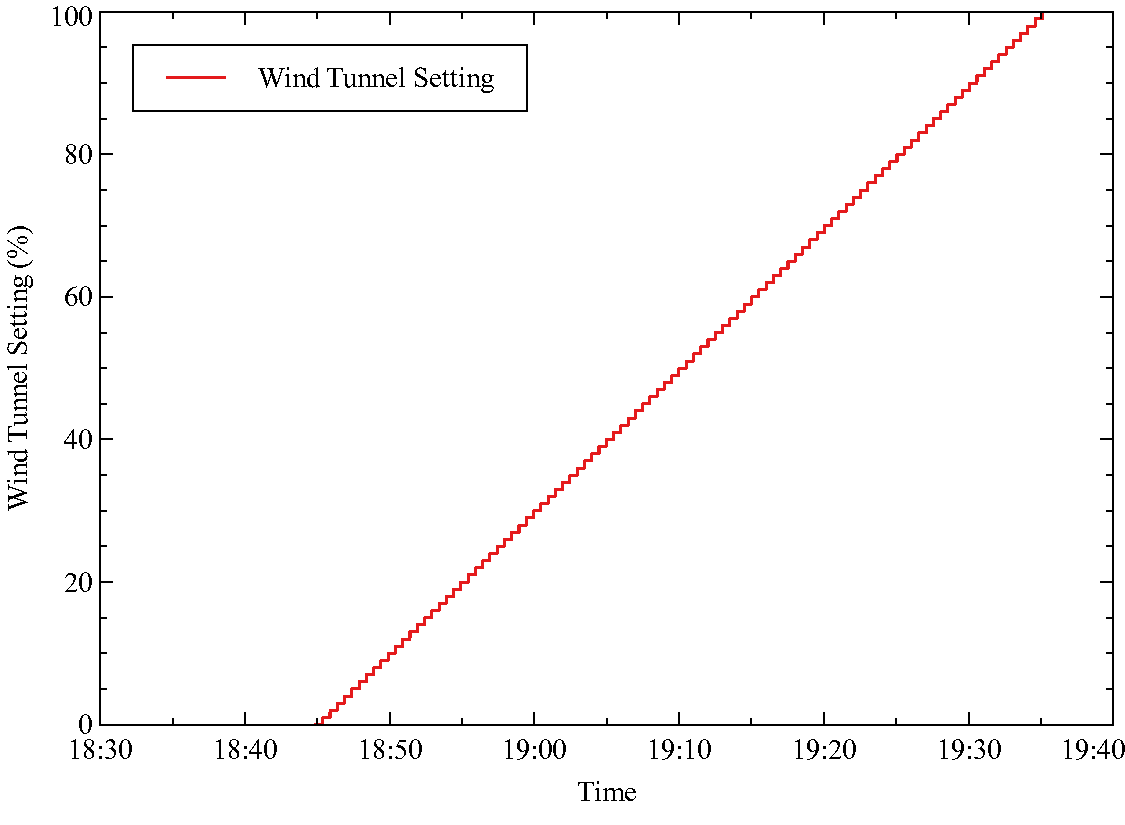
\includegraphics[width=0.9\textwidth]{cardCalibration_01}
	\caption{Wind Tunnel Setting}
	\label{fig:tunnelSetting}
\end{figure}

\noindent
The velocity in the wind tunnel as recored by the hot wire anemometer and results from the pitot static tube based on Equation \ref{simplifiedPhysicsFt} are shown in Figure \ref{fig:rawVelocity}.  The results shown here (and used in subsequent analysis) are an average of 10 seconds of data centered on the middle of the wind tunnel speed steps shown in Figure \ref{fig:tunnelSetting}.  The 10 second subset of data was selected to avoid velocity instabilities in the wind tunnel immediately after wind tunnel setting changes.

\begin{figure}[H]
	\centering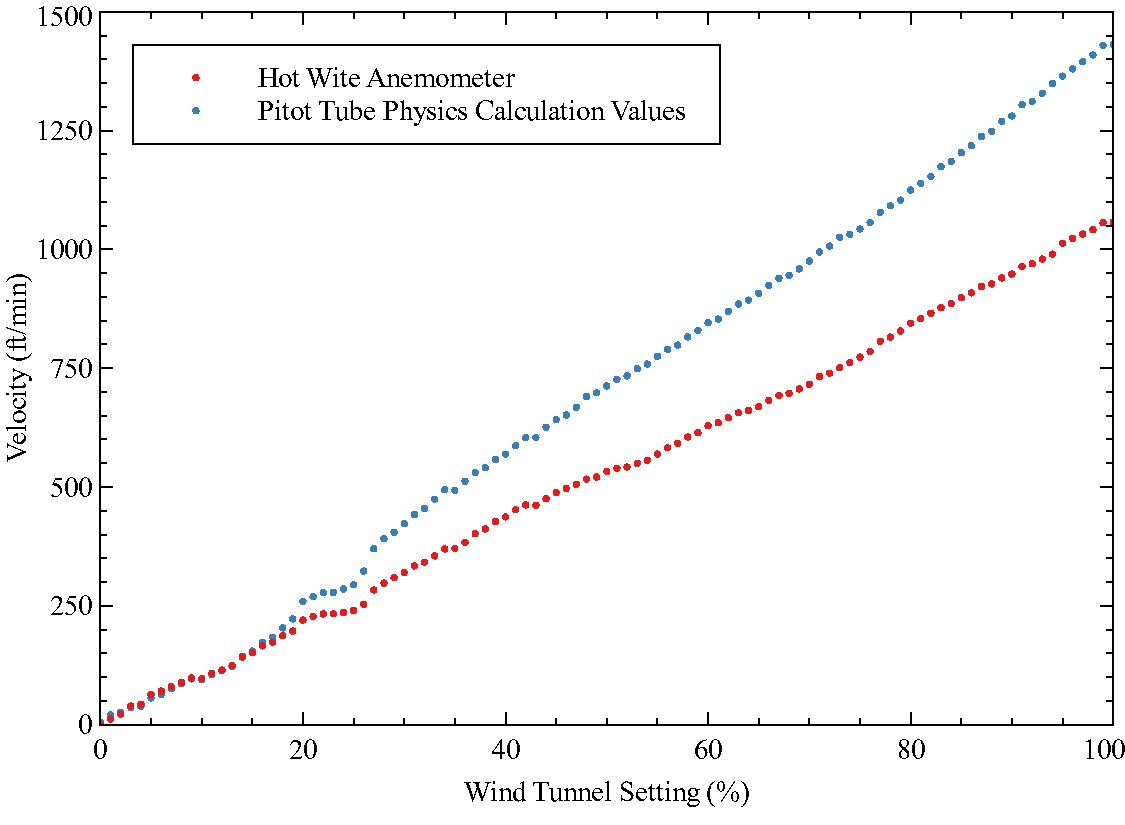
\includegraphics[width=0.9\textwidth]{cardCalibration_04}
	\caption{Uncalibrated Velocity}
	\label{fig:rawVelocity}
\end{figure}

\noindent
Figure \ref{fig:calibration} shows the physics based calculation of velocity relative to readings from the hot wire anemometer.  This relation was used to create a two part curve fit to calibrate the pitot static tube results with the hot wire anemometer results.  The correlation is linear for velocities above $362.645 \frac{ft}{min}$.  Below that point, the pitot static tube response is non-linear and fit with a second order polynomial.  

\begin{figure}[H]
	\centering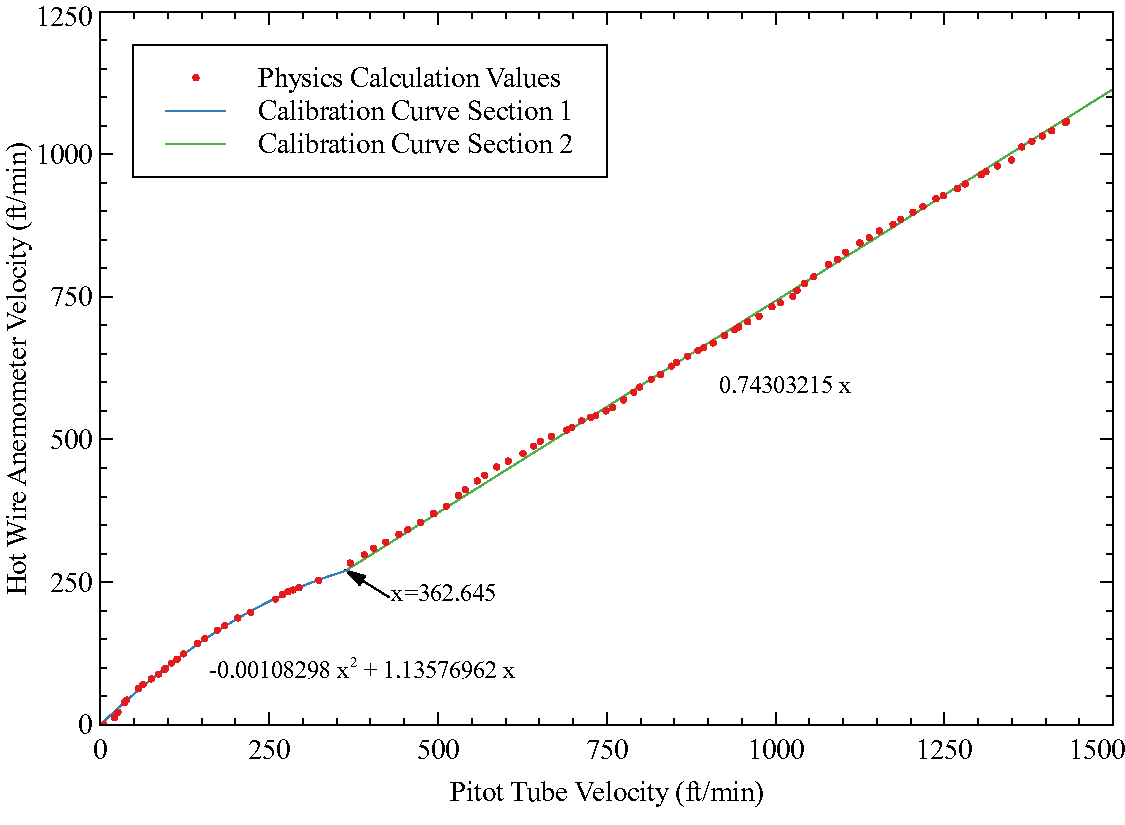
\includegraphics[width=0.9\textwidth]{cardCalibration_02}
	\caption{Pitot Tube Calibration Curves}
	\label{fig:calibration}
\end{figure}

\noindent
Figure \ref{fig:result} shows the calibrated velocity results.  In this image, the $1:1$ Line shows an ideal fit between the two parameters.  When the airflow velocity is less than approximately $30 \frac{ft}{min}$ the pitot static tube provides unreliable results (with errors up to $93\%$).  Beyond this lower threshold the average error is $1.02\%$ and the maximum error is $4.59\%$.

\begin{figure}[H]
	\centering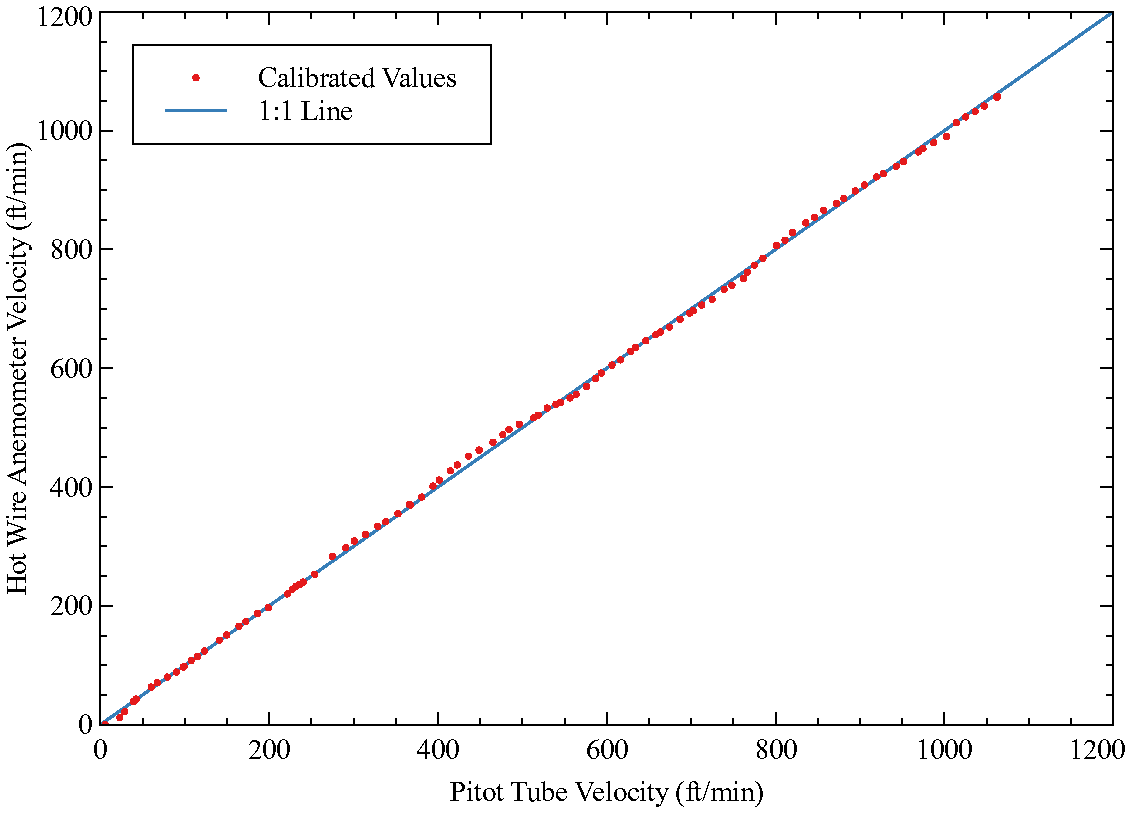
\includegraphics[width=0.9\textwidth]{cardCalibration_03}
	\caption{Calibration Result}
	\label{fig:result}
\end{figure}

\end{document}
